The concrete syntax used to declare an \emph{association} in CML
is specified by listing \ref{lst:stx:association}.
First, the \textbf{association} keyword is followed by a NAME.
Then, a list of \emph{association ends} are declared under the \textbf{association} block.
For each declaration of an \emph{association end},
The \textbf{conceptName} and \textbf{propertyName} are optionally followed by a \textbf{typeDeclaration}.

\begin{code}
\verbatimfont{\small}
\lstinputlisting[language=antlr]{grammar/Associations.txt}
\caption{Association Concrete Syntax}
\label{lst:stx:association}
\end{code}

The \emph{Association} metaclass is presented
in the EMOF \cite{mof} class diagram of figure \ref{fig:meta:association},
and its instantiation from the concrete syntax is specified by listing \ref{lst:ast:associations}.
For each parsed \emph{association},
an instance of the \emph{Association} metaclass will be created,
and its meta-properties will be assigned
according to parsed information:

\begin{itemize}

\item \emph{name}:
assigned with the value of the token NAME.

\item \emph{members}:
an \emph{ordered set} referencing all \emph{associationEnd}
instances parsed in the \textbf{association} block.

\end{itemize}

\begin{code}
\verbatimfont{\small}
\lstinputlisting[language=lsl]{ast/associations.lsl}
\caption{Association AST Instantiation}
\label{lst:ast:associations}
\end{code}

\begin{figure}
\centering
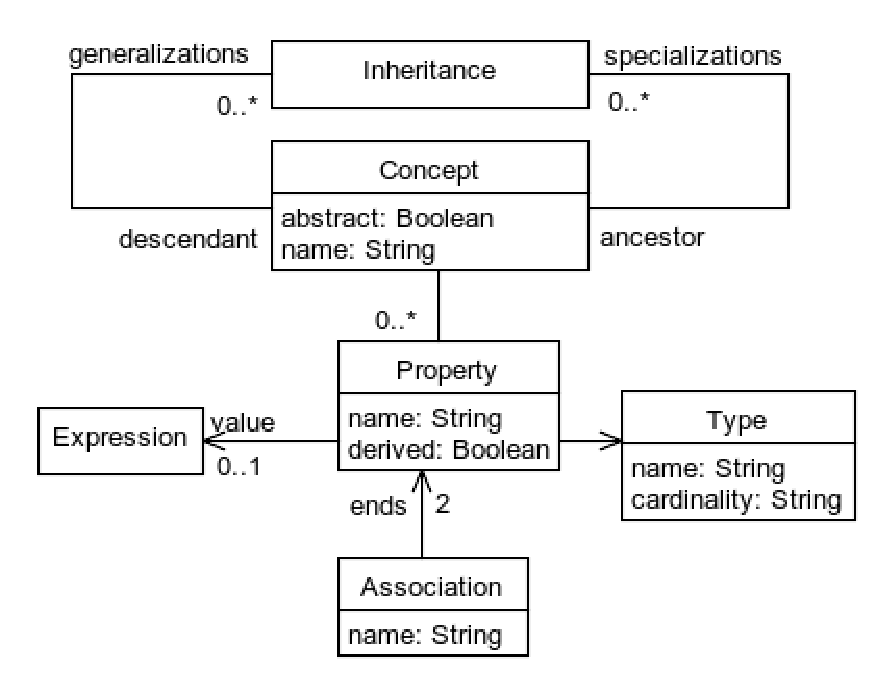
\includegraphics[width=1.0\textwidth]{metamodel/association}
\caption{Association Abstract Syntax}
\label{fig:meta:association}
\end{figure}
